\chapter{Estudos de Caso} \label{ch:cdu}

O presente capítulo visa explicar os estudos de caso utilizados para validar o
sistema desenvolvido. Todo experimento foca no agente que possui uma parte escrita em
\emph{AgentSpeak} para decidir como as percepções se ligam com a ontologia
afetiva, os limites da emoção virar sentimento deve ser decidido inicialmente
e o agente deve receber uma percepção ``step'' quando for um novo ciclo de
simulação para recalcular os sentimentos.

Os experimentos são simulações de parte da vida dos personagens. No primeiro, eles
encontram-se observando um jogo de futebol e cada um torce por um time. No
segundo, uma casa é simulada com quatro atores e suas rotinas. Entretanto,
antes desses estudos serem abordados na seção~\ref{ch:cdu:svc} e na
\ref{ch:cdu:home}, será descrito como a ontologia foi testada juntamente com a
plataforma \emph{Jason}. A seção~\ref{ch:cdu:tbc} explica as ferramentas
desenvolvidas para o teste da base de crenças desenvolvida e são duas: uma
interativa e outra não interativa que serve como uma espécie de teste unitário
dos artefatos explicados no capítulo~\ref{ch:aec}.

\section{Teste da Base de Crenças} \label{ch:cdu:tbc}

Os testes da base de crenças têm como finalidade checar se a utilização normal
está acontecendo da maneira esperada. Assim, eles fazem testes de inserção,
recuperação, remoção e listagem. Os testes foram escritos na linguagem
\emph{AgentSpeak}.

\begin{figure}
	\begin{center}
		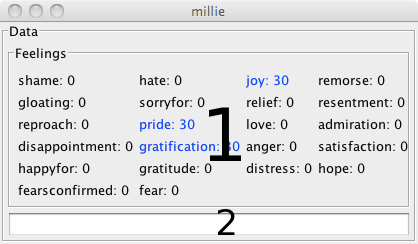
\includegraphics[width=70mm]{figuras/introductionDF.png}
	\end{center}
	\caption{Interface para mostrar os sentimentos dos agentes.}
	\label{fig:introducaoDF}
\end{figure}

A primeira aplicação de teste desenvolvida foi de maneira interativa conforme
pode ser observado na Figura~\ref{fig:introducaoDF}. A aplicação permite que o
usuário escreva as crenças do agente em um campo texto (área 2 na figura) e
esse é enviado diretamente para a base de crenças do agente. Na área 1 da mesma
figura a valência das emoções é mostrada.
Essas informações podem aparecer em: preto, se não houve alteração com o ciclo
anterior; azul, se houve um aumento; vermelho, se houve uma diminuição do
valor.

\begin{figure}
	\begin{center}
		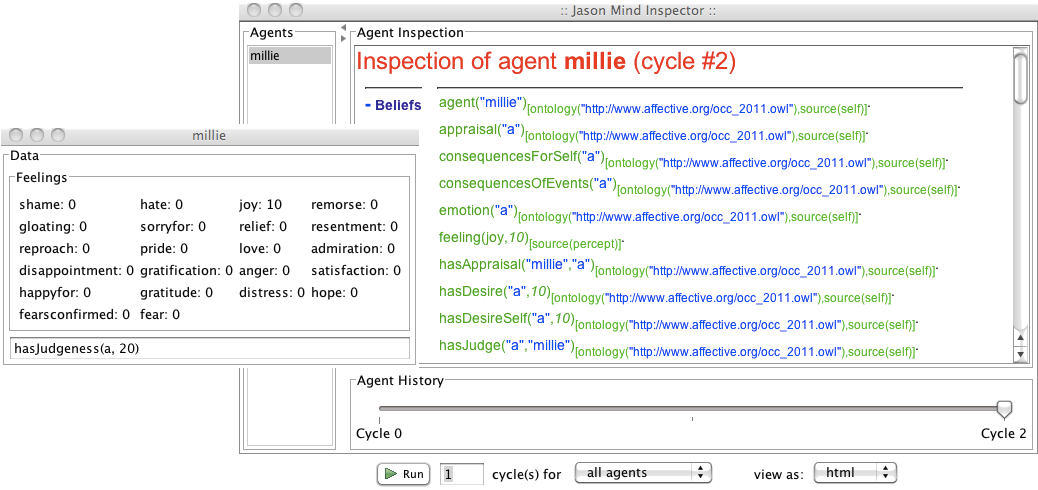
\includegraphics[width=150mm]{figuras/beforeLastInsertionOfPride.png}
		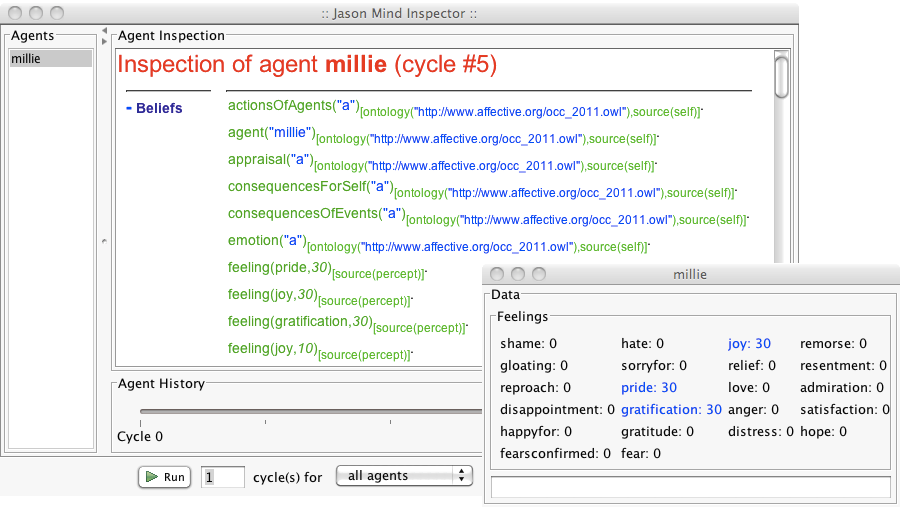
\includegraphics[width=150mm]{figuras/afterLastInsertionOfPride.png}
	\end{center}
	\caption{Exemplo de utilização criando uma emoção de orgulho.}
	\label{fig:testeJasonIntBase}
\end{figure}

Na Figura~\ref{fig:testeJasonIntBase} estão representados dois momentos da
criação de uma emoção de orgulho pelo usuário. Na parte de cima, o
agente tem configurado uma avaliação de e sobre si próprio. Além disso, a
avaliação tem probabilidade nula ou irrelevante e o desejo para si mesmo foi
considerado com o valor 10. Esse valor poderia ser qualquer número inteiro,
mas se fosse negativo ao invés de alegria (\emph{joy}) o resultado atual seria
sofrimento (\emph{distress}).

Na parte de baixo da Figura~\ref{fig:testeJasonIntBase} está o resultado
obtido após a inserção da última crença para criação da emoção de orgulho.
Conforme pode ser visto, foi necessário três ciclos deliberativos para o
agente ter a percepção do sentimento. Note que essa percepção do sentimento,
não veio do simulador e sim de o agente erroneamente acreditar que existe um
passo de simulação novo e então disparar o processo emotivo para criar as emoções
conforme configuração. Se fosse um passo normal da simulação, não se
teria na base de crenças duas percepções \emph{feeling} sobre uma emoção
porque a todo novo ciclo as percepções são apagadas. Cabe chamar atenção que
no sistema desenvolvido não existe o decaimento dos valores com o
passar do tempo, para isso ser feito o agente deve reavaliar o problema e
atualizar os valores nas suas crenças.

Na Listagem~\ref{lst:testeJasonIntBase} pode ser observada uma configuração
para rodar o presente aplicativo\footnote{Veja a seção
\ref{sec-jason-overview} na página~\pageref{sec-jason-overview}
para ver uma introdução sobre esse tipo de arquivo.}. O ambiente na linha 3
espera que todos os agentes (quantidade informada no parâmetro 3) mandem
uma ação para prosseguir. O simulador espera por essas ações pelo tempo em milissegundos
configurado no primeiro parâmetro, caso não venha ignora o
agente e segue para o próximo ciclo. O segundo parâmetro permite informar
um número que representa o último passo de simulação e o quarto
parâmetro permite configurar a atitude a ser tomada quando um agente tentar
fazer duas ações no mesmo passo. Essa atitude pode ser ou o enfileiramento da
ação ou a falha imediata da mesma que é a utilizada no exemplo.

\begin{center}
    \begin{minipage}{130mm}
	\lstset{linewidth=130mm}
	\lstinputlisting[frame=trbl, caption=Arquivo de projeto do \jason para a aplicação interativa de teste., label=lst:testeJasonIntBase]{../../sampletConsole/eoaus.mas2j}
    \end{minipage}
\end{center}

O agente configurado da linha 5 à 9 utiliza opções do \jason para
alterar a base de crença sendo utilizada (\emph{beliefBaseClass}),
arquitetura (\emph{agentArchClass}) e o raciocinador
(\emph{agentClass}). As classes dessas alterações foram explicadas anteriormente
na seção~\ref{ch:p:ipjo}~(pág.~\pageref{ch:p:ipjo}).
Assim, para o presente exemplo a mudança da arquitetura na linha 7, única
classe não mencionada até agora, foi realizada para criar e atualizar a janela
mostrada na Figura~\ref{fig:testeJasonIntBase} que exibe os dados emotivos.

Na linha 6 da Listagem~\ref{lst:testeJasonIntBase} foi incluída somente
a ontologia afetiva desenvolvida. Assim, para o agente
utilizar as emoções ainda é necessário incluir as configurações de ativação
dos sentimentos via código. Uma amostra do código utilizado para se fazer isso
pode ser vista na Listagem~\ref{lst:testeJasonIntSetup} que mostra algumas
crenças iniciais do agente.

As crenças iniciais são carregadas no agente no inicio da simulação. O processo
de carga segue conforme determinado na classe da linha 6 da
Listagem~\ref{lst:testeJasonIntBase}. Sendo assim, a crença ``step'' como não
consta na ontologia será carregada na base de crenças padrão e as demais serão
criadas na base de conhecimento. Esse processo fica transparente
para o código \emph{AgentSpeak}, porém o usuário precisa definir para as 22
emoções o limite mínimo para as mesmas serem percebidas como sentimento.

\lstset{linewidth=80mm}
\begin{wrapfigure}{l}{80mm}
	\begin{lstlisting}[frame=trbl,
caption=Parte do código do agente para aplicação interativa de teste.,
label=lst:testeJasonIntSetup]
step(0)[source(percept),source(self)].

agent(millie).

hasSetup(millie, setup1).
hasThreshold(setup1, 0).
hasThresholdType(setup1, "Joy").

hasSetup(millie, setup2).
hasThreshold(setup2, 0).
hasThresholdType(setup2, "Distress").
	\end{lstlisting}
\end{wrapfigure}

Nesse exemplo, os valores de limites estão sendo configurados com valoração
zero para que a potência e a valência sejam iguais. O agente somente conhece
a valência de uma emoção que é o valor da potência menos o limite de
ativação. Entretanto, tanto o limite de ativação quanto a potência não são
conhecidos pelo agente. Por exemplo, se o limite da pena (\emph{sorryFor}) é 6
e o valor atual é 8 então o sentimento de pena terá valor 2 sendo
expresso por uma crença da seguinte forma ``feeling("sorryFor",2).''.

%%%% fim da explicacao da aplicação interativa %%%%%

A aplicação não interativa utiliza a configuração do arquivo de projeto mostrado no
Apêndice~\ref{atni} (pág.~\pageref{atni}).
O ambiente especificado na linha 4 possui os mesmos
parâmetros do anterior com o acréscimo de um novo que indica uma ontologia.
Essa serve para o ambiente conhecer as rotinas dos agentes, como
deve ser desenhado o mapa a ser exibido e as posições iniciais de cada
agente. O agente millie aqui é o utilizado para os testes e os limiares de
ativação de emoção estão configurados para valores diferentes. Existe uma
variedade de testes para as propriedades de objeto ou de dados e para as
instâncias de classes, além de testes das conclusões esperadas.

\section{Assistindo um jogo de futebol} \label{ch:cdu:svc}

O caso de uso apresenta dois personagens que estão no mesmo lugar e assistindo ao mesmo jogo de
futebol. O jogo tem ao todo 60 turnos que representam os 90 minutos de um jogo
regulamentar. Em cada turno é sorteado um número randômico com probabilidade
de 1.67\% para os times marcarem gol, isto é, há 98.33\% de
chance a cada turno de nada acontecer e o placar permanecer inalterado.

Esse exemplo aparentemente simples, propicia um cenário bastante rico para as
emoções porque um personagem pode ter diferentes emoções acontecendo.
Essas emoções são muitas vezes do ramo de consequências de eventos por
estar ligada com a desejabilidade do evento ou do ramo de ações de agentes que
tem a ver com a responsabilidade das ações. Assim, as mentes dos atores que estão
assistindo ao jogo de futebol decidem no inicio da simulação os nomes de seus
times e ambos acreditam que vencerão.

O arquivo de projeto dessa aplicação pode ser consultada no Apêndice~\ref{adps}
(pág.~\pageref{adps}) e cria dois agentes:
``watch1'' e ``watch2''. Cada um com seu próprio código fonte e,
dessa forma, cada um deles inclui em seus códigos as configurações
necessárias para utilizar o sistema. Um exemplo dessas configurações
é o limite de ativação para uma emoção virar sentimento. Outro exemplo é que
os times que participam do jogo são considerados pelos personagens como outros
agentes, assim o time pode ser considerado ``amigo'' e o outro ``inimigo''.

Cabe salientar que cada um dos agentes realizam as mesmas avaliações sobre os
mesmos eventos. Esses eventos foram pensados como a marcação de um gol
(Listagem~\ref{lst:soccerGoal}), o estado atual do jogo
(Listagem~\ref{lst:soccerTeam}) e  o estado final do jogo
(Listagem~\ref{lst:soccerEnd1} e Listagem~\ref{lst:soccerEnd2}).
Esses são alguns exemplos escritos na plataforma \jason para
fins de validação.

\begin{center}
    \begin{minipage}{120mm}
	\lstset{linewidth=120mm}
	\begin{lstlisting}[frame=trbl,
caption=Parte do código do agente referente à avaliação de gol.,
label=lst:soccerGoal]
+?appraisalGoal
    :  goal(TEAM) & myPoints(TEAM, PF, _, _)
    <- ?fib(8-(PF+1), VAL);
       ?updateEmotion(prospectIrrelevant, "goal_myteam_pi", VAL);
       +removeEmotion("goal_myteam_pi").

+?appraisalGoal
    :  goal(TEAM) & myPoints(_, _, TEAM, PE)
    <- ?fib(PE+1, VAL);
       ?updateEmotion(prospectIrrelevant, "goal_enemyteam_pi", -VAL);
       +removeEmotion("goal_enemyteam_pi").

+?appraisalGoal
    : removeEmotion(INDIVIDIDUAL)
   <- ?removeEmotion(prospectIrrelevant, INDIVIDIDUAL);
      -removeEmotion(INDIVIDIDUAL).

+?appraisalGoal.
	\end{lstlisting}
    \end{minipage}
\end{center}

A Listagem~\ref{lst:soccerGoal} realiza o processamento das emoções sentidas
por um personagem quando um time marca um gol. Cada um dos planos criados
visam atender as 4 condições possíveis: gol do meu time, gol do adversário,
gol que não é mais percebido e não houve gols. O plano da
linha 4 (\emph{updateEmotion}) e o da linha 15 (\emph{removeEmotion}, não
confundir o plano com a crença) serão explicados adiante, por hora basta saber
que eles atualizam ou removem as relações necessárias para a afetividade.

Na última listagem mencionada, as linhas 3 e 9 chamam um plano que consulta os números de
\emph{fibonacci}. Esse plano tem no primeiro parâmetro a posição do número na
sequência e o retorno correspondente.
Os times quando jogam no simulador dificilmente
marcam mais que 5 gols então foi decidido limitar os números de
\emph{fibonacci} até a sétima posição. Valores de posição negativos ou
superiores à 7 terão retorno um. Quando um gol é marcado
a favor do time que o agente torce o \emph{fibonacci} é usado de maneira
decrescente, isto é, o primeiro gol retornará a sétima posição, o segundo à
sexta e etc. No caso de gols do time adversário é utilizado o cálculo de
\emph{fibonacci} de maneira crescente. Logo, o valor 1 é retornado para os
dois primeiros gols, o terceiro valor 2 e assim por diante.

A Listagem~\ref{lst:soccerTeam} é similar à anterior. Ela é responsável por inserir uma
emoção de esperança no agente com valoração 50 e inicia o cálculo de
performance do evento assumindo o valor positivo 1. Cada gol percebido
do próprio time incrementa esse valor em 10 e quando o gol é do
adversário é feito um decremento no mesmo valor. A emoção de esperança não
sofre alteração depois que é criada porque esta sendo considerado que as
emoções são baseadas na percepção dos eventos ou ações. Dessa forma, a esperança do
jogo ser ganho só termina quando há a percepção do encerramento do mesmo e a
performance do evento que foi calculada é utilizada nesse momento.

\begin{center}
    \begin{minipage}{130mm}
	\lstset{linewidth=130mm}
	\begin{lstlisting}[frame=trbl,
caption=Parte do código do agente referente ao andamento do jogo.,
label=lst:soccerTeam]
+?appraisalTeam
    :  not(hasLikelihood("team_hope_prn", PROB)) & step(STEP) & STEP < 10
    <- ?updateEmotion(prospectNotRealized, "team_hope_prn", 50);
       +realizedCalculation(1).

+?appraisalTeam
    :  goal(TEAM) & myPoints(_,_, TEAM, _) // ponto que nao eh meu
    &  realizedCalculation(CALC)
    <- -realizedCalculation(CALC);
       +realizedCalculation(CALC-10).

+?appraisalTeam
    :  goal(TEAM) & myPoints(TEAM, _, _,_) // ponto que eh meu
    &  realizedCalculation(CALC)
    <- -realizedCalculation(CALC);
       +realizedCalculation(CALC+10).

+?appraisalTeam.
	\end{lstlisting}
    \end{minipage}
\end{center}

\begin{center}
    \begin{minipage}{140mm}
	\lstset{linewidth=140mm}
	\begin{lstlisting}[frame=trbl,
caption=Parte do código do agente referente à avaliação do final do jogo para
as emoções de probabilidade.,
label=lst:soccerEnd1]
+?appraisalEndMatch
    :  realizedCalculation(CALC) & match(_,_)
    &  hasLikelihood("team_hope_prn", PROB)
    &  feeling(hope, HOPEVAL)
    <- ?removeEmotion(prospectNotRealized, "team_hope_prn");
       ?updateEmotion(prospectRealized, "team_satisfaction_pr", HOPEVAL, CALC);
       -realizedCalculation(CALC).

+?appraisalEndMatch
    :  realizedCalculation(CALC) & match(_,_)
    &  hasLikelihood("team_hope_prn", PROB)
    <- ?removeEmotion(prospectNotRealized, "team_hope_prn");
       -realizedCalculation(CALC).

+?appraisalEndMatch.
	\end{lstlisting}
    \end{minipage}
\end{center}

Nas Listagens~\ref{lst:soccerEnd1}~e~\ref{lst:soccerEnd2} são realizadas
avaliações depois do termino do jogo. O jogo pode terminar empatado ou um dos
dois times ganhar. Entretanto, para a primeira listagem basta que o jogo tenha
terminado para uma atitude ser tomada. Essa atitude é a remoção da emoção de
esperança e a criação de uma nova emoção baseado em como foi o andamento do
jogo e no valor atual da esperança. Sendo assim, um personagem pode ficar
satisfeito ou desapontado.

Já, a Listagem~\ref{lst:soccerEnd2} permite um personagem sentir-se feliz
por ou com pena do resultado de seu time. Quando o time do personagem
tiver ganho o jogo ele pode sentir-se feliz ou neutro e quando o time perde
ele pode sentir-se com pena ou neutro da mesma forma. Esse valor de
neutralidade é porque o modelo de emoções só diz que a felicidade por alguém
ou a pena serão sentidas quando o merecimento e o desejo presumido sobre o
outro forem ambas positivas ou negativas.

\begin{center}
    \begin{minipage}{140mm}
	\lstset{linewidth=140mm}
	\begin{lstlisting}[frame=trbl,
caption=Parte do código do agente referente à avaliação do final do jogo para
as emoções relacionadas com a consequência de eventos para outros.,
label=lst:soccerEnd2]
+?appraisalEndMatchHappy
     : match(win, TEAM) & myPoints(TEAM, _, _, _)
     & not(hasAppraisal(NAME, "team_happy_foo"))
    <- .random(N); DE=math.round(N*20)-10; DT=20;
       ?updateEmotion(fortunesOfOthers, "team_happy_foo", DE, DT).

+?appraisalEndMatchHappy
     : match(lose, TEAM) & myPoints(TEAM, _, _, _)
     & not(hasAppraisal(NAME, "team_happy_foo"))
    <- .random(N); DE=math.round(N*20)-10;
       DT=-20; // eh negativo para implicar na emocao de pena
       ?updateEmotion(fortunesOfOthers, "team_happy_foo", DE, DT).

+?appraisalEndMatchHappy
     : match(draw, _) & myPoints(TEAM, _, _, _)
     & not(hasAppraisal(NAME, "team_happy_foo"))
    <- .random(N); DE=math.round(N*20)-10; DT=10;
       ?updateEmotion(fortunesOfOthers, "team_happy_foo", DE, DT).

+?appraisalEndMatchHappy.
	\end{lstlisting}
    \end{minipage}
\end{center}

As consultas de ``removeEmotion'', presentes nas listagens anteriores, recebem
o grupo emotivo e o nome do indivíduo que deve ser removido. Com base nessas
informações, as relações que foram outrora inseridas são removidas da
ontologia e, consequentemente, da base do \jason normal. Um exemplo é mostrado
na Listagem~\ref{lst:removeSample} no qual são removidas as relações: de
merecimento, de desejo por outros, de qual pessoa está sendo avaliada e de
quem está avaliando.

As consultas de ``updateEmotion'' funcionam de maneira parecida à
``removeEmotion'' e fazem a inserção de relações. Caso já exista o
indivíduo, removem e acrescentam novas relações para alterar o valor guardado.
Dessa forma, para a construção do exemplo tanto as atualizações como as
remoções foram agrupadas por grupo de emoções visto que essa é a forma que
o próprio modelo \occ agrupa as emoções com regras similares. A Listagem~\ref{lst:update}
mostra as regras para o grupo emotivo que tem a ver com a consequência dos
destinos dos outros, isto é, as relações de merecimento, de nível de
desejo presumido e de quem está avaliando e de qual pessoa está sendo
avaliada.

\begin{center}
    \begin{minipage}{130mm}
	\lstset{linewidth=130mm}
	\begin{lstlisting}[frame=trbl,
caption=Amostra de remoção de emoção do tipo destino de outros.,
label=lst:removeSample]
+?removeEmotion(fortunesOfOthers, INDIVIDUAL)
     : hasDeserved(INDIVIDUAL, OLDDE) & hasDesireOther(INDIVIDUAL, OLDDO)
     & hasPerson(INDIVIDUAL, TEAM)
    <- ?myName(NAME);
       -hasPerson(INDIVIDUAL, TEAM);
       -hasDeserved(INDIVIDUAL, OLDDE);
       -hasDesireOther(INDIVIDUAL, OLDDO);
       -hasAppraisal(NAME, INDIVIDUAL).

+?removeEmotion(fortunesOfOthers, INDIVIDUAL).
	\end{lstlisting}
    \end{minipage}
\end{center}

\begin{center}
    \begin{minipage}{130mm}
	\lstset{linewidth=130mm}
	\begin{lstlisting}[frame=trbl,
caption=Amostra de código referente as atualizações de emoções do tipo destino
de outros.,
label=lst:update]
+?updateEmotion(fortunesOfOthers, INDIVIDUAL, DESERVED, DESIREOTHER)
     : team(TEAM) & not(hasPerson(INDIVIDUAL, TEAM))
    <- ?myName(NAME);
       +hasAppraisal(NAME, INDIVIDUAL);
       +hasPerson(INDIVIDUAL, TEAM);
       +hasDeserved(INDIVIDUAL, DESERVED);
       +hasDesireOther(INDIVIDUAL, DESIREOTHER).

+?updateEmotion(fortunesOfOthers, INDIVIDUAL, DESERVED, DESIREOTHER)
     : hasDeserved(INDIVIDUAL, OLDDE) & hasDesireOther(INDIVIDUAL, OLDDO)
    <- -hasDeserved(INDIVIDUAL, OLDDE);
       +hasDeserved(INDIVIDUAL, DESERVED);
       -hasDesireOther(INDIVIDUAL, OLDDO);
       +hasDesireOther(INDIVIDUAL, DESIREOTHER).

+?updateEmotion(fortunesOfOthers, INDIVIDUAL, DE, DO).
	\end{lstlisting}
    \end{minipage}
\end{center}

\section{Simulando uma casa} \label{ch:cdu:home}

O presente estudo de caso tem por finalidade demonstrar as ontologias de rotinas
e preferências trabalhando junto da afetividade. Ele utiliza o ambiente e os
agentes de maneira diferente do caso anterior. O agente aqui não carrega os
limites de ativação dos sentimentos de crenças iniciais e, sim, da própria
ontologia. Todos seus valores estão configurados para a emoção virar
sentimento a partir do valor 20\label{mark:emo} por simplicidade, mas poderiam ter qualquer
valor configurado pelo usuário.

O ambiente utilizado nesse exemplo foi explicado brevemente quando foi introduzido o
aplicativo de teste não-interativo. Esse ambiente carrega uma ontologia que
tem por finalidade conhecer as preferências e as rotinas dos agentes e
disponibilizá-las na forma de percepções aos agentes, além de
construir uma visualização do ambiente onde é possível visualizar os atores
desses agentes atuando. As percepções nesse ambiente são apagadas e criadas
novamente em cada passo de simulação.

Para a construção da visualização, cada um dos indivíduos do conceito
\emph{Place} são considerados como objetos que devem ser desenhados se
estiverem associados à uma dimensão. Assim, todos os objetos na tela são
desenhados a partir de retângulos. Além disso, esse conceito pode usar a
relação \emph{hasSetup} visando determinar que um objeto tem determinada
anotação ou, ainda, determinar que objetos fazem parte de um objeto maior.
Para o ambiente é importante conhecer as anotações dos objetos porque
quando esses objetos são percebidos pelo agente vai junto as anotações
que esses objetos possuem. Por exemplo, o objeto ``camaSolteiro1'' tem as
anotações de posição nos eixos x e y, tamanhos nos dois eixos, utilidade
``dormir'' e dono um ou mais personagens.

Cabe chamar atenção que o personagem em nenhum momento recebe a informação
do ambiente de onde ele se encontra. Essa informação o agente descobre baseado
na percepção do ambiente. Por exemplo, o agente sabe que o ``quarto1'' possui
um armário, dois criados mudos, duas camas e duas portas. O agente sabe o nome
correto de cada um dos itens que estão no quarto então ele pode a partir da
percepção buscar em seu mapa onde os objetos que percebe estão e então
concluir que ele se encontra em uma determinada sala. Assim, usando o
conhecimento extraído de um objeto que possui outros objetos, ele é capaz de
construir um mapa mental com a finalidade principalmente de se localizar e
saber quais objetos ele deve alcançar para chegar em um destino. Mas, esse
mapa não carrega consigo as informações de anotações que só são obtidas via
percepção. Dessa forma, um ator precisa a primeira vez descobrir qual é a sua
cama e onde ela se encontra quando quiser descansar.

\begin{figure}
	\begin{center}
		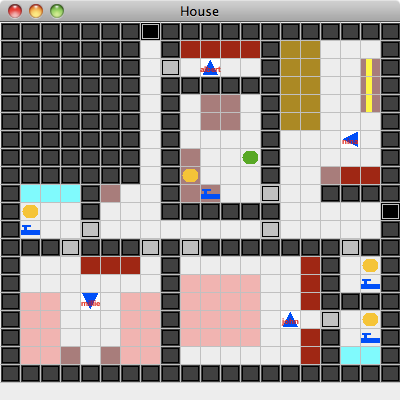
\includegraphics[width=10cm]{figuras/sims.png}
	\end{center}
	\caption{Interface de visualização da casa sendo simulada.}
	\label{fig:sims}
\end{figure}

A Figura~\ref{fig:sims} possui quatro atores diferentes chamados: Millie,
Albert, Nina e John. Esses atores estão localizados inicialmente em diferentes
pontos da casa e cada um possui uma orientação própria. No inicio da simulação eles
devem averiguar os objetos próximos para perceberem em qual sala se encontram
e depois decidem um objetivo próprio baseado em seu estado interno atual.
Esse estado interno encontra-se representado por uma característica
fundamental que é a energia que o ator possui para gastar e todos os agentes
iniciam com ela no valor 40 podendo a mesma ir de 0 a 100. Sendo
assim, muito provavelmente no inicio da simulação os agentes tentarão ir
descansar em suas respectivas camas para obter energia para o dia seguinte.

O valor de energia mencionando antes é informado pelo ambiente ao
agente. Cada um dos agentes recebe uma percepção sobre seu estado
interno que foi denominada ``myself''. O agente usa essa informação junto de
sua preferência pelas anotações para determinar que emoção ele irá sentir.
Quando o valor de energia está abaixo de um determinado limite estipulado pela
preferência da anotação de energia o agente começa a ter um
determinado nível de sofrimento. No caso de ele estar com a energia acima do
limite, o mesmo possuirá a emoção que corresponde à alegria.

Esse exemplo simples com duas emoções serve para demonstrar o uso de todas as
ontologias desenvolvidas. Sendo assim, o ambiente possui 206 indivíduos com
aproximadamente 70\% deles sendo necessários para a criação dos 60 objetos
presentes na tela (paredes, mesa, camas, etc). A
Figura~\ref{fig:abstractWindow} mostra na esquerda o mapa abstrato que o agente
pode consultar via ação interna e a direita o mapa da visualização.

\begin{figure}
	\begin{center}
		%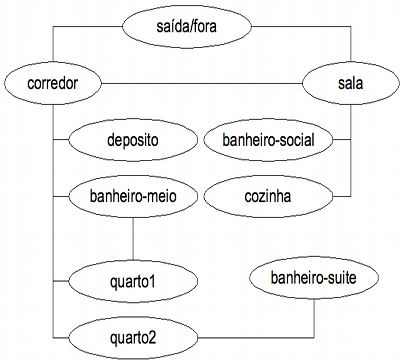
\includegraphics[width=70mm]{figuras/abstract.png} % esquerda
		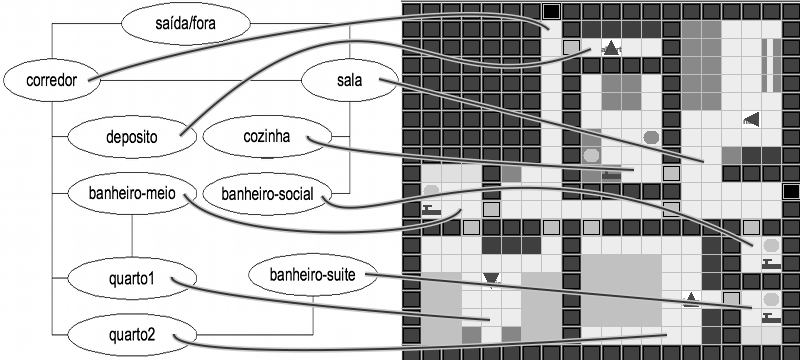
\includegraphics[width=140mm]{figuras/visualization.png}
	\end{center}
	\caption{Mapa do agente (esquerda) e visualização (direita).}
	\label{fig:abstractWindow}
\end{figure}

A Figura~\ref{fig:abstractWindow} é útil para entender a forma como o agente
conhece a casa. Esse grafo é utilizado pelo mesmo para ir de um lugar para
outro. Assim, este é construído antes da simulação iniciar, a partir dos dados
da ontologia informada para o ambiente. Entretanto, esse mapa possui somente
os itens (Figura~\ref{fig:abstractAnother} adiante) de cada lugar e não possui nenhum conhecimento das anotações.
Além disso, essas informações são disponibilizadas por ações
internas: retornar todos os itens, retornar todos os cômodos, retornar o
cômodo de determinado item ou retornar todos os itens de um cômodo.

Conforme dito anteriormente, a primeira coisa que o agente faz é descobrir
onde ele se encontra. Assim, quando o agente entra em uma sala, ele busca por
todos os itens que ele percebe por duas razões. Primeira, é para manter uma
lista dizendo a orientação e o que foi percebido lá. A segunda razão é que
quando o agente não sabe onde se encontra, o mesmo pergunta ao ambiente a
localização de todos os itens percebidos e a localização mais citada é a
considerada atual. Isso é necessário porque mesmo havendo obstáculos que o
agente não consegue passar ou ver, algumas vezes objetos de outros lugares são
percebidos. Por exemplo, o agente que inicia no norte (depósito) quando olha
para o sul pode perceber a mesa (cozinha).

O mapa abstrato mostrado na Figura~\ref{fig:abstractWindow} é apresentado
com os respectivos itens em suas respectivas localizações na
Figura~\ref{fig:abstractAnother}. Novamente, esse mapa é montado antes do
inicio da simulação conforme configuração da ontologia informada no
ambiente. Além disso, as posições iniciais dos personagens também encontram-se
configurados nesta juntamente com seus perfis.

\begin{wrapfigure}{l}{9cm}
	\begin{center}
		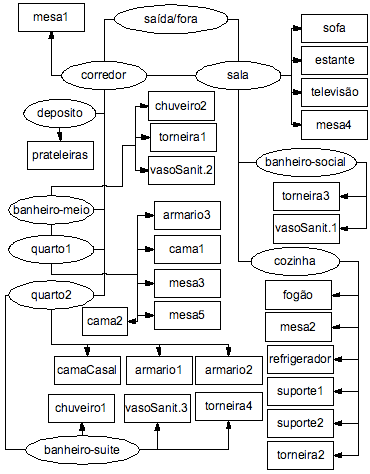
\includegraphics[width=7cm]{figuras/abstract-comitens.png}
	\end{center}
	\caption{Grafo usado para descobrir os itens.}
	\label{fig:abstractAnother}
\end{wrapfigure}

Esses perfis são usados para definir a rotina diária de um ator porque eles
permitem relacionar estabelecimentos como destinos possíveis ou fixos.
Assim, ao todo existem 4 perfis configurados, dois para estudantes e
outros dois para trabalhadores. Os estudantes vão para escola pela manhã e
após possuem destinos eventuais. Enquanto um dos perfis vai eventualmente ao
mercado, o outro vai ao fliperama. O perfil ``trabalhador'' tem o local de
trabalho como fixo e o mercado como eventual. Já o último perfil está sendo
considerado como um trabalhador caseiro. Dessa forma, ele não possui nenhum
destino fixo, somente destinos eventuais.

Os locais existentes são, basicamente, a casa, a escola, o fliperama, o
mercado e o trabalho. Desses locais, a casa é a única visualizada por ser o
local que os agentes passam a maior parte de seu tempo e tempos de abertura e
fechamento não são aplicáveis. A Tabela~\ref{tab:estaloca} mostra os horários
de funcionamento dos estabelecimentos. Os horários estão no formato 0-23
horas, sendo que ``-'' significa que não abre naquele dia. Além disso, os
horários são em formato texto porque são passados os horários para todos os
dias da semana. A semana esta sendo considerada como iniciando em uma
segunda-feira e terminando no domingo. Fora isso, os locais marcados como
fixos são locais que o agente deve permanecer até que o horário de
funcionamento termine. Já os considerados eventuais pode se ir algumas vezes
e ficar por um tempo indeterminado.

\begin{table}[h]
	\caption{Horário de funcionamento dos estabelecimentos.}
	\label{tab:estaloca}
	\begin{center}
	\begin{tabular}{|c|c|c|}
	%\begin{tabular}{|p{34mm}|p{50mm}|p{50mm}|}
		\hline
		Local & Abertura & Encerramento \\ \hline
		Casa & X & X \\ \hline
		Escola & 7,7,7,7,7,-,- & 11,11,11,11,11,-,- \\ \hline
		Fliperama & 15,15,15,15,15,9,8 & 21,21,21,21,21,21,21 \\ \hline
		Mercado & 7,7,7,7,7,7,8 & 21,21,21,21,21,20,19 \\ \hline
		Trabalho & 8,8,8,8,8,-,- & 17,17,17,17,17,-,- \\ \hline
	\end{tabular}
	\end{center}
\end{table}

As preferências do agente sobre as anotações estão sendo usadas para ajudar o
agente a decidir o que fazer. Elas permitem o agente sentir-se ou alegre ou
sofrer. Basicamente, cada um dos agentes tem seu próprio conjunto de
preferências. Entretanto, o presente exemplo irá focar somente na anotação de
energia. Cada um dos agentes é atraído por uma valoração positiva desse valor.
Por exemplo, o limite de Albert é 50. John é 55. Millie é 30 e Nina é 53.

Esses valores de limite permite a aplicação determinar quando uma emoção será
sentida. Para Albert o valor 50 é o ponto médio de energia no qual ele não
sente nenhuma emoção e qualquer valor acima ou abaixo disso ocasiona uma
emoção que pode virar sentimento. Dessa forma, quando Albert passar a ter 71 de energia
ele passará a experimentar alegria. De forma igual, quando Millie atingir o
valor 9 de energia estará sentindo sofrimento. O valor de 71 e 9 são
justificados porque o processo de avaliação os cria com base nas preferências as
emoções. Albert, quando a energia está em 71, possui a emoção de alegria no
valor 21. Sendo assim, o agente experimenta o sentimento de alegria com valor
1 porque o limite para uma emoção virar sentimento esta configurada com o
valor 20 (pág.~\pageref{mark:emo}). A mesma coisa acontece com o agente Millie,
sua energia está no valor 9 que garante a emoção de sofrimento com valor 21 e
a percepção da emoção com valor 1.

O presente exemplo possui 4 agentes que compartilham o mesmo código
\emph{AgentSpeak}. Entretanto, as suas bases de crenças estão configuradas com
ontologias diferentes. Assim, eles têm diferentes crenças iniciais sem
precisar escrever código. O processo de deliberação inicia avaliando a
percepção de energia, se ela chegou em zero então o personagem é removido da
visualização. Depois, é feita a avaliação das emoções e um comportamento é
escolhido.

\begin{figure}
\begin{center}
    \begin{minipage}{130mm}
	\lstset{linewidth=130mm}
	\begin{lstlisting}[frame=trbl,
caption=Amostra de código referente ao processo de avaliação considerando as
preferências.,
label=lst:appraisal]
+?appraisal
    <- .findall(prRe(A,P), priority(repulse, A, P), LRE);
       .findall(prAt(A,P), priority(attract, A, P), LAT);
       .findall(OBJ, OBJ[source(percept)], PERCEPTS);
       ?appraisalPercept(PERCEPTS, LRE, LAT).

+?appraisalPercept([], LRE, LAT).
+?appraisalPercept([PERCEPT|R], LRE, LAT)
     : PERCEPT =.. [FUNCTOR,TERMS,_]
    <- ?appraisalPercept(R, LRE, LAT);
       .findall(X, PERCEPT[X], ANNOTS);
       ?appraisalOnePercept(PERCEPT, ANNOTS, LRE, VALR);
       ?appraisalOnePercept(PERCEPT, ANNOTS, LAT, VALP).

+?appraisalOnePercept(_, _, [], 0).
+?appraisalOnePercept(PERCEPT, ANNOTS, [PR|L], NEWVAL)
    <- ?appraisalOnePercept(PERCEPT, ANNOTS, L, VAL);
       ?appraisalOneAnnotation(ANNOTS, PR, VAL, NEWVAL);
       ?evalAppraisal(PERCEPT, PR, VAL, NEWVAL).

+?appraisalOneAnnotation([], _, VAL, VAL).
+?appraisalOneAnnotation([H|R], PR, OLDVAL, NEWVAL)
     :  H =.. [NAMEPRI,          [VALTER|_], _]
     & PR =.. [FUNCPRI, [NAMEPRI,PARTPRI|_], _]
    <- ?appraisalOneAnnotationValue(VALTER, PARTPRI, FUNCPRI, OLDVAL, VAL);
       ?appraisalOneAnnotation(R, PR, VAL, NEWVAL).
+?appraisalOneAnnotation([H|R], PR, OLDVAL, NEWVAL)
    <- ?appraisalOneAnnotation(R, PR, OLDVAL, NEWVAL).
	\end{lstlisting}
    \end{minipage}
\end{center}
\end{figure}

No inicio da simulação, a base de crenças converte os itens guardados na
ontologia como preferências para crenças no formato ``priority(Type,
Annotation, Partition)''. Assim, o processo pega todas essas crenças em duas listas
e cria uma lista de objetos percebidos e as envia para a próxima etapa
que recupera todas as anotações de um objeto e realiza o cálculo baseado nas
prioridades do que é importante. A Listagem~\ref{lst:appraisal} mostra esse
procedimento, o operador ``=..'' é usado para desmanchar a variável em uma
lista com três elementos: o termo, os parâmetros e as anotações.

O cálculo que dispara as emoções baseando-se nas preferências do indivíduo é
realizado pela consulta ``appraisalOneAnnotationValue''. Essa consulta recebe
por parâmetro: o valor da anotação; o valor de limite da mesma; seu tipo
(atração por números abaixo ou acima do limite); valor atual das anotações do
objeto; e, o resultado do cálculo. Esse cálculo pode ser visto na
Listagem~\ref{lst:anotcalc}.

\begin{figure}
\begin{center}
    \begin{minipage}{130mm}
	\lstset{linewidth=130mm}
	\begin{lstlisting}[frame=trbl,
caption=Amostra de código referente ao cálculo de uma anotação.,
label=lst:anotcalc]
// NUMBER
+?appraisalOneAnnotationValue(VALT, VALP, _, OLDV, NEWV)
     : .number(VALT) & .number(VALP) & VALT = VALP
    <- NEWV = OLDV.
+?appraisalOneAnnotationValue(VALT, VALP, prRe, OLDV, NEWV)
     : .number(VALT) & .number(VALP) & VALT < VALP
    <- NEWV = OLDV+(VALP-VALT).
+?appraisalOneAnnotationValue(VALT, VALP, prRe, OLDV, NEWV)
     : .number(VALT) & .number(VALP) & VALT > VALP
    <- NEWV = OLDV+(VALP-VALT).
+?appraisalOneAnnotationValue(VALT, VALP, prAt, OLDV, NEWV)
     : .number(VALT) & .number(VALP) & VALT > VALP
    <- NEWV = OLDV+(VALT-VALP).
+?appraisalOneAnnotationValue(VALT, VALP, prAt, OLDV, NEWV)
     : .number(VALT) & .number(VALP) & VALT < VALP
    <- NEWV = OLDV+(VALT-VALP).

// ATOM
+?appraisalOneAnnotationValue(VALT, VALT, FUNCTOR, OLDV, OLDV+1)
     : .atom(VALT).
+?appraisalOneAnnotationValue(VALT, VALP, FUNCTOR, OLDV, OLDV)
     : .atom(VALT) & .atom(VALP).
	\end{lstlisting}
    \end{minipage}
\end{center}
\end{figure}

Esse processo leva em consideração o tipo da anotação sendo analisada. Por
exemplo, elas podem ser números ou átomos. O cálculo verifica se os dois
valores informados nos dois primeiros parâmetros são iguais, se for então o
resultado é a devolução do valor antigo. No caso de ser uma preferência por
negativa então o segundo parâmetro que é o valor informado na ontologia é
subtraído do primeiro parâmetro que é o valor atual ou observado da anotação.
No caso de ser uma preferência positiva então o valor atual da anotação é
subtraído do valor informado.

O processo de atualização de emoções é disparado pela consulta
``evalAppraisal'' presente na Listagem~\ref{lst:appraisal} na linha 19.
Essa consulta recebe como parâmetro: a percepção; a crença de prioridade;
o valor anterior; e, o valor calculado das anotações presentes na percepção.
Assim, a consulta ``evalAppraisal'' é utilizada para averiguar os dados antes
de ocorrer a chamada à consulta ``updateEmotion'' que é similar a explicada
anteriormente. O código dessa consulta está apresentado na
Listagem~\ref{lst:acEmotion} e é responsável simplesmente por construir o
nome do indivíduo usando o termo da percepção e o valor informado na ontologia.

\begin{figure}
\begin{center}
    \begin{minipage}{130mm}
	\lstset{linewidth=130mm}
	\begin{lstlisting}[frame=trbl,
caption=Amostra de código referente à atualização das emoções.,
label=lst:acEmotion]
+?evalAppraisal(_, _, OLDVAL, OLDVAL).
+?evalAppraisal(PCP, PREF, OLDVAL, NEWVAL)
     : PCP =..  [FUNCP,         [], _]
     & PREF =.. [FUNCF, [TERM1F|_], _]
     & NEWVAL > 0
    <- .concat("", FUNCP, "_", TERM1F, INDIVIDUAL);
       ?updateAppraisal(joy, INDIVIDUAL, NEWVAL).
+?evalAppraisal(PCP, PREF, OLDVAL, NEWVAL)
     : PCP =..  [FUNCP,         [], _]
     & PREF =.. [FUNCF, [TERM1F|_], _]
     & NEWVAL < 0
    <- .concat("", FUNCP, "_", TERM1F, INDIVIDUAL);
       ?updateAppraisal(distress, INDIVIDUAL, NEWVAL).
	\end{lstlisting}
    \end{minipage}
\end{center}
\end{figure}

